\chapter{Weakly Supervised Object Segmentation}

Most algorithms for semantic image segmentation and object-class segmentation
work with strong supervision: a pixel-wise labeling of training images. In this
chapter, we investigate a method that works with annotation that is much
easier to obtain: whole image labels.
While we do not reach the accuracy of competing fully supervised approaches,
our efficient, semi-supervised method is potentially able to scale to much
larger datasets, without the need of time-consuming manual annotation on
pixel-level.

Recently, several approaches have been proposed for semi-supervised semantic
segmentation.  While these are close to our work, there are several important
distinctions.  We address the task of object-class segmentation, that concerns
object categories, while semantic segmentation approaches often focus on
"stuff" categories like "sky" and "road" that are more easily detected using
simple texture features.
Additionally, in contrast to \citet{vezhnevets2011weakly}, our approach is in
principle applicable to large datasets, the regime where weak annotation is
most useful.

In our approach, we work with a set of candidate segments, generated using
constrained parametric min-cuts~\citep{carreira2010constrained}.  For each
image, these segments are a set of overlapping, object-like regions, which
serve as candidates for object locations.

We formulate weakly supervised multi-class image segmentation as a
multi-instance problem, based on these candidate segments.  In multi-instance
learning~\citep{dietterich1997solving}, each training example is given as a
multi-set of instances, called a bag.  Each instance is represented as a
feature vector $x$ and a label $y$.

A bag is labeled positive if it contains at least one positive example, and
negative otherwise.  During training, only the labels of the training bags, not
of the instances inside the bags, are known.  The goal is to learn a classifier
for unseen bags. 
Formally, let $\mathcal{X}$ be the set of instances. To simplify notation, we
assume that bags are simply sets, not multi-sets.  Then a bag is an element of
the power set $2^\mathcal{X}$ and the task is to learn a function
\begin{equation} f_{MI} \colon 2^\mathcal{X} \rightarrow \{-1,+1\}.  \end{equation}
Training examples are tuples $(X_i,y_i)$ of bags $X_i \subset \mathcal{X}$ and
labels $y_i \in \{-1,+1\}$.  It is assumed that the $f_{MI}$ function stems
from a so-called underlying concept, given by an (unknown) function
$f_{I} \colon \mathcal{X} \rightarrow \{-1,+1\}$, with 
\begin{equation}\eqlabel{multi_instance}
f_{MI}(X)= \max_{x \in X}\ f_{I}(x).
\end{equation}

Multi-instance learning is a natural formulation for image classification and
has been successfully applied in this task~\citep{zhou2007multi}. We propose to
go a step further and apply multi-instance learning to the task of object-class
segmentation in natural images, by also classifying instances, not only bags.
In this, we follow the work of \citet{liconvex2010} and \citet{zha2008joint}, who not
only learn $f_{MI}$, but also $f_{I}$.

In our model, each image forms a bag, while the candidate segments correspond
to the instances contained in the bag. During learning, only presence of object
classes is needed as bag level supervision. By learning $f_{I}$, we are then
able to predict for individual segments whether they contain the object class
of interest, thereby obtaining a segmentation of the object.
To measure the performance of our algorithm, we use a dataset that not only contains
image level annotation, but also pixel level annotation of object. This allows
us to judge the succes of learning on instance level.

\section{Related Work}
\subsection{Proposal Object Segments}\label{related_segments}
Most work on multi-class segmentation focuses on strong supervision on
superpixel level. There is still little work on using candidate segments.  The
method we use for generating candidate segments is Constraint Parametric
Min-Cuts (CPMC) from \citet{carreira2010constrained}.  This method creates a
wide variety of overlapping segments. Support vector regression (SVR) is
trained on these segments to estimate the overlap of segments with ground truth
object-class labeling from the Pascal VOC dataset~\citep{pascal}. This provides
a ranking of candidate segments, according to how ``object-like'' they are,
which allows for selecting only a limited number of very object-like segments.
The method performed well on a variety of datasets. A similar approach was
investigated by \citet{endres2010category}.
%Brendel and Todorovic~\citet{NIPS2010_0122} also use a set of candidate segments is used, though all of these are kept throughout the whole 
%algorithm.

\subsection{Multi-Instance Methods}
Multi-instance learning was formally introduced in \citet{dietterich1997solving}.
Since then, many algorithms were proposed to solve the multi-instance learning problem
\citep{andrews2003support,gaertner2002multi,zhou2009multi,li2009convex,zhang2002dd,mangasarian2008multiple,leistner2010miforests,chen2006miles}.
We discuss only those that are relevant to the present treatment.

\citet{gaertner2002multi} introduced the concept of a multi-instance
kernel on bags, defined in terms of a kernel on instances. 
The basic principle of the multi-instance kernel is similar to a soft-max over instances in
each bag. This can be viewed as approximating the kernel value of the ``closest pair'' given by two bags. \citet{gaertner2002multi} show that the multi-instance kernel
is able to separate bags if and only if the original kernel on instances is able to separate the underlying concepts.
The method of multi-instance kernels has a particular appeal in that it transforms a multi-instance problem into a standard
classification problem by using an appropriate kernel. The downside of this approach is that it does
not directly label instances, only bags.
 %and that it assumes that instances inside a bag have i.i.d.
%labels.

\citet{zhou2009multi} explicitly address the fact that instances are not
independent within a bag , leading to an algorithm that can take advantage of
possible correlations. Computational costs of their algorithm does not scale
well with the number of instances, although a heuristic algorithm is proposed
to overcome this restriction. 
%FIXME where does this sentence go?
\citet{zhou2009multi} demonstrated only a slight
advantage of their algorithm over the MI-kernel of \citet{gaertner2002multi},
so we use the MI-kernel for better scalability.

\citet{liconvex2010} compute likelihood ratios for instances, giving a new
convex formulation of the multi-instance problem. Using these likelihood
ratios, classification can be performed directly on the instances, provided an
appropriate threshold for classifying instances as positive is known. We
circumvent this problem by applying the same classifier to instances and bags,
thereby obtaining hard class decisions for each instance.

%\subsection{Multi Instance Multi Label (MIML) Methods}
%Zhou and Zhang~\citet{zhou2007multi} were some of the first to tackle the problem of multi-instance multi-label tasks.
%They proposed two methods, MIMLBoost and MIMLSvm. MIMLBoost transforms a MIML task into
%a multi-instance learning task by reformulating the problem of \Eqref{miml} as
%\begin{equation} f_{MIL} \colon 2^\mathcal{X}\times \mathcal{Y} \rightarrow \{ -1, +1\}.\end{equation}
%This corresponds to learning a single multi-instance classifier per class.
%MIMLSvm, on the other hand, transforms a MIML task into a multi-label task by constructing a mapping
%\begin{equation} \phi \colon 2^\mathcal{X} \rightarrow \mathcal{Z} \end{equation}
%into a new instance space $\mathcal{Z}$ by medioid clustering.
%Our approach fits well into the category of MIMLBoost: we also transform the MIML task
%into a multi-instance task that we then solve using MI-kernels.
%While our problem formulation is similar to Zhou and Zhang, we aim not only at image classification but
%also at object segmentation.

%Zha\etal\citet{zha2008joint} use a Hidden Conditional Random Field (HCRF), directly capturing the semantics of each instance.
%The HCRF model used is a complex probabilistic model that in practice can only be trained using contrastive divergence.
%For inference, Gibbs sampling is used, making recall very time consuming.
%Nguyen~\citet{nguyen2010new} proposed an iterative algorithm for MIML that alternates between phases of label propagation, in which
%labels are assigned to instances, and margin-maximization, in which feature weights are adjusted.

%The algorithms of Zha and Nguyen have the benefit of explicitly exploiting correlations between labels.
%It is noteworthy, however, that both rely heavily on approximate optimizations. We concentrate our efforts
%on methods that are faster and scale better with the number of instances and bags.

%In our work, we demonstrate how a computationally efficient algorithm combined with strong object segmentation hypotheses can efficiently solve MIML
%tasks as they occur in weakly supervised multi-class image segmentation, using only a single convex optimization.

\subsection{Semantic Scene Segmentation using Weak Annotation}
Learning semantic segmentation from image-level annotation was first investigated in \citet{verbeek2007region},
using a semi-supervised conditional random field on patches. \citet{verbeek2007region} evaluated their approach
on the MSRC-9 datasets.
More recently, simliar approaches were proposed by
\citet{vvezhnevets2011weakly} and \citet{vezhnevets2010towards}.
\citet{vezhnevets2011weakly} independently developed a multiple-instance based
approach to segmentation, and report impressinve results on the MSRC-21 dataset.

While semantic segmentation is closely related to multi-class image
segmentation, there are important distinctions: In semantic segmentation, each
pixel has a semantic annotation, also containing non-object ``stuff'' classes like
``sky'', ``grass'' and ``water''. In multi-class image segmentation, the focus
is on objects, with possibly large parts of the image being labeled as
unspecific ``background''.  The unspecific background class contains much more
clutter than for example ``grass'' and is therefore much harder to model. Additionally,
object classes themselves are much harder to capture using low-level textural information only.
This makes disseminating the distinctive features in multi-class object recognition
much more challenging.


\section{Multi-Instance Kernels for Image Segmentation}
\subsection{Constraint Parametric Min Cuts (CPMC)}
% Repetition?
To generate proposal segments, we use the Constraint Parametric Min Cut (CPCM)
method from \citet{carreira2010constrained}. In CPMC, initial segments are
constructed using graph cuts on the pixel grid. The energy function for these cuts
uses pixel color and the response of the global probability of boundary (gPb)
detector~\citep{maire2008using}. As much as ten thousand initial segments are
generated from foreground and background seeds. A fast rejection based on
segment size and ratio cut~\citep{wang2003image} reduces these to about 2000
overlapping segments per image. Then, the segments are ranked according to a
measure of object-likeness that is based on region and Gestalt properties.
This ranking is computed using an SVR model~\citep{carreira2010constrained},
which is available online. 
% TODO implementation detail?
For computing the global probability of boundary
(gPb), we used the CUDA implementation of \citet{catanzaro2009efficient}, which
provides a speedup of two orders of magnitude over the original implementation.

\subsection{Multi-Instance Learning using MI-Kernels}
Since scalability is very important in real-world computer vision applications,
and natural images might need hundreds of segments to account for all possible
object boundaries, we use the efficient multi-instance
kernels~\citep{gaertner2002multi}.  Multi-instance kernels are a form of set
kernels %TODO add reference to earlier work -> convolution kernel
 that transform a kernel on instance level to a kernel on bag level.  We
reduce the multi-instance multi-class problem to a multi-instance problem by
using the one-vs-all approach.

With $k_I$ denoting a kernel on instances $x,x' \in \mathcal{X}$, we define the
corresponding multi-instance kernel $k_{MI}$ on bags $X,X' \in 2^\mathcal{X}$
as
\begin{equation}\eqlabel{mi_kernel}
k_{MI}(X,X') := \sum_{x \in X, x' \in X'} k^p(x,x'),
\end{equation}
where $p \in \mathbb{N}$ is a free parameter~\citep{gaertner2002multi}. As we use
the RBF-kernel $k_{rbf}$ as kernel on $\mathcal{X}$ and powers of RBF-kernels
are again RBF-kernels, we not consider $p$ explicitly in the following.

We normalize the kernel $k_{MI}$ \citep{gaertner2002multi} using
\begin{equation}
k(X,X') := \frac{k_{MI}(X,X')}{\sqrt{k_{MI}(X,X)k_{MI}(X',X')}}.
\end{equation}
Training an SVM with this kernel produces a bag-level classifier for each
class, which we refer to as MIK\@.  This procedure is very efficient since
the resulting kernel matrix is of size number of bags, which is much smaller
than a kernel matrix of size number of instances, as is commonly used in the
literature~\citep{andrews2003support,nguyen2010new,zhang2008m3miml}.  Another
advantage over other methods is, that it uses a single convex optimization,
whereas other approaches often use iterative
algorithms~\citep{andrews2003support} or need to fit complex probabilistic
models~\citep{zha2008joint}.

While using MIK has many advantages, it produces only an instance-level
classifier. We propose to transform a bag-level classifier $f_{MI}$ as given by
the SVM and \Eqref{mi_kernel} into an instance-level classifier by setting
$f_{I}(x):=f_{MI}(\{x\})$, in other words, by considering each instance as its own
bag. 
We extend the MIK SVM to the multi-class case using the one-vs-rest approach,
learning one SVM for each class.

\subsection{Segment Features}

To describe single segments, we make use of densely computed
SIFT~\citep{lowe2004distinctive} and ColorSIFT~\citep{van2009evaluating}
features, from which we compute bag of visual word histograms. Additionally, we
use histograms of oriented gradients~\citep{dalal2005histograms} on the
segments.  We use RBF-kernels for all of the features, constructing one
MI-kernel per feature. These are then combined using multiple kernel learning
to produce a single kernel matrix. This kernel matrix can then be used for all
classes, making classification particularly efficient.

\subsection{Combining Segments}\seclabel{combiningsegments}

The framework described above yields an image-level and a segment-level
classification. In our setup, each segment might be given multiple labels.
To obtain a pixel-level object-class segmentation, we have to combine these.
As each image in the training set contains only a single class, we only consider the class
predicted by the bag-level one-vs-rest classifier.
Since we do not make use of the ground truth segmentation during training, we cannot learn an optimal
combination as in \citet{li2010object} but perform a simple majority vote
instead.  We merge segments into pixel-level class labels by setting the label
$y_x$ of a pixel $x$ according to
\begin{equation}
    y_x = \argmax_{y \in Y} \#\{S_i | p \in S_i \land y_{S_i}=y \},
\end{equation}
where $Y$ is the set of possible object classes, $S_i$ enumerates all segments within an
image and $y_{S_i}$ is the label of segment $S_i$. In words: each pixel is
assigned the class with the highest number of class segments containing it.
This simple heuristic yields good results in practice.

\begin{figure}[tbp]
	\begin{center}
        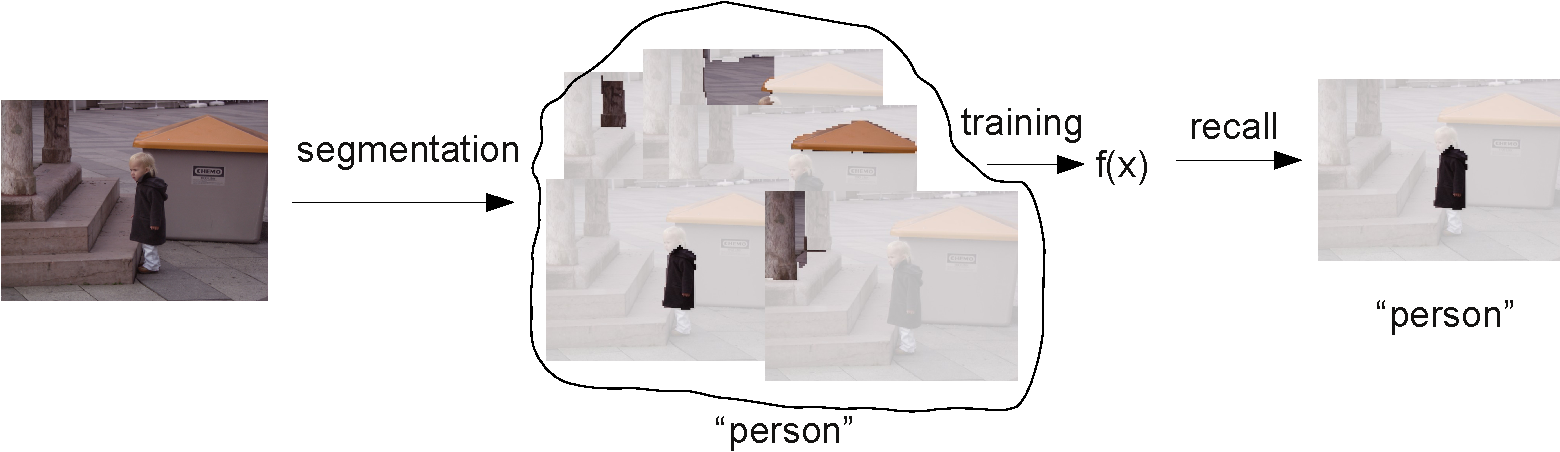
\includegraphics[width=\linewidth]{images/scheme-crop.pdf}
	\end{center}
        \caption{Overview of our method. See text for details.}
	\figlabel{results}
\end{figure}

\section{Experiments}

\subsection{Instance-Level Predictions using MI-Kernel}

To assess the validity of instance-level predictions using multi-instance
kernels, we transform $f_{I}$ back to an instance-level classifier, using the
multi-instance learning assumption (\Eqref{multi_instance}). We refer to these
instance-based MIK predictions as MIK-I. In all experiments, the
parameters of the MI-Kernel and SVM are adjusted using MIK and then used with
both MIK and MIK-I.  This facilitates very fast parameter scans since
MIK is very efficient to compute. Note that we cannot adjust parameters using
instance prediction error, as we assume no instance labels to be known.

\begin{table}
    \centering
    \begin{tabularx}{\linewidth}{@{\extracolsep{\fill}}lccccccc}
    \toprule
        & SVM-SVR & EMDD & mi-SVM & MI-SVM & MICA & MIK & MIK-I \\
    \cmidrule(rl){2-8}
    Musk1 & 87.9 &84.9 &  87.4 &  77.9     & 84.3 & 88.0& 88.0 \\
    Musk2 & 85.4 &84.8 &  83.6 &  84.3     & 90.5 & 89.3& 85.2 \\
    \bottomrule
    \end{tabularx}
    \caption{Bag level performance of various MIL algorithms on the standard Musk
    datasets. All but MIK provide instance-level labeling.\tablabel{muskacc}}
    
\end{table}
We compared the performance of MIK, MIK-I and state-of-the-art MI
methods on the Musk benchmark datasets~\citep{dietterich1997solving}, see
\Tabref{muskacc}. Results were obtained using 10-fold cross-validation. While
the computational complexity of MIK-I is very low compared to the other
methods, it achieves competitive results.  Using instance-level labels results
in a slight loss of accuracy of MIK-I, compared to MIK\@. This small
degradation of performance is quite surprising, since the model was not trained
to provide any instance-level labels.

For multi-class image segmentation, it is beneficial to have a low witness
rate, that is only a few instances are assumed to be positive in a positive
bag. Since an object might not be very prominent in an image, only a fraction
of segments might correspond to the object.
\Tabref{musk-witness} compares the witness rates of MIK-I,
miSVM~\citep{andrews2003support} and SVR-SVM~\citep{liconvex2010} on the Musk
datasets. MIK-I is able to achieve similar accuracy with much less
witnesses than the other methods.  Note that Musk1 consists of very small bags
while Musk2 contains significantly larger bags, more similar to the
image/segment setup.

\begin{table}
    \centering
    \begin{tabularx}{\linewidth}{@{\extracolsep{\fill}}lcccc}
    \toprule
    & \multicolumn2c{Musk1}  & \multicolumn2c{Musk2}  \\
                &accuracy & witness-rate & accuracy & witness-rate  \\
    \cmidrule(rl){2-3}
    \cmidrule(rl){4-5}
    mi-SVM      & 87.4          & 100\%               &  83.6          & 83.9\%\\
    SVM-SVR     & 87.9          & 100\%               &  85.4          & 89.5\%\\
    MIK-I& 88.0          & 99\%                &  85.2          & 62.3\%\\
    \bottomrule
    \end{tabularx}
    \caption{MIL algorithms and the empirical witness rates of the
        classifiers.  \tablabel{musk-witness}}
\end{table}

\subsection{Partially Supervised Image Segmentation on Graz 02}

We evaluate the performance of the proposed algorithm for object-class
segmentation on the challenging Graz-02 dataset.  This dataset contains 1096
images of three object classes, bike, car and person.  Each image may contain
multiple instances of the same class, but only one class is present per image.

We adjusted parameters on a hold-out validation set using bag-level information
and used the training and test sets as given by the dataset.  It is
straight-forward to extend the binary MIK method to the multi-class setting
using a one-vs-all strategy.
We train one multiple kernel learning (MKL) SVM per class using MIK and predict
class labels on segment level using MIK-I. If at least one SVM
classifies a segment as positive, it is associated with the most confident
class. Otherwise, it is assigned ``background'' or no class.
This yields a classification of each segment into one of four classes: car,
bike, person, or background. We merge segments into pixel-level class labels as
described in \Secref{combiningsegments}.

\begin{figure}[tbp]
	\begin{center}
        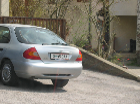
\includegraphics[width=35mm]{images/car1_img.png}\hspace*{0.7ex}
        
\includegraphics[width=35mm]{images/car1_gt.png}\hspace*{0.7ex}
        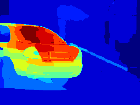
\includegraphics[width=35mm]{images/car1_pos.png}\hspace*{0.7ex}
        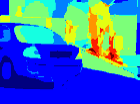
\includegraphics[width=35mm]{images/car1_neg.png}\hspace*{0.7ex}\\
        \vspace{1mm}
        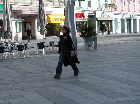
\includegraphics[width=35mm]{images/person1_img.png}\hspace*{0.7ex}
        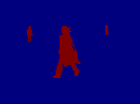
\includegraphics[width=35mm]{images/person1_gt.png}\hspace*{0.7ex}
        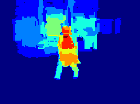
\includegraphics[width=35mm]{images/person1_pos.png}\hspace*{0.7ex}
        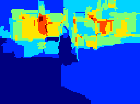
\includegraphics[width=35mm]{images/person1_neg.png}
	\end{center}
        \caption{Qualitative results on on the Graz-02 dataset. Top: Results on
        category ``car''. Bottom: Results on category ``person''. From left to
        right: original image, ground truth segmentation, segment votes for
        correct class, segment votes against correct class (red many, blue few votes).}
	\figlabel{results}
\end{figure}

\begin{table}
    \centering
    \begin{tabularx}{\linewidth}{@{\extracolsep{\fill}}p{208pt}ccc}
    \toprule
                & car & bike & person \\
    \cmidrule(l){2-2}
    \cmidrule(l){3-3}
    \cmidrule(l){4-4}
        This work&   0.30&  0.45&  0.43 \\
        Best strongly supervised approaches~\citep{fulkerson2009class,schulz2011}&   0.72&  0.72&  0.66 \\
    \bottomrule
    \end{tabularx}
    \caption{Pixel-level accuracy on the Graz-02 dataset.
        \tablabel{tab:graz}}
\end{table}

Per-class pixel accuracies are reported in \Tabref{tab:graz}; some qualitative
results are shown in \Figref{results}. The overall accuracy on images labels,
which is the task that was actually trained, is $90\%$.  While the performance
of our multiple-instance based approach is far from current methods that use
pixel-level annotations, whose pixel-level accuracy is around
$70\%$~\citep{fulkerson2009class,schulz2011} on pixel-level, it can serve as a
baseline for research on weakly supervised methods for object-class segmentation.

\section{Summary}

We proposed an algorithm for object-class segmentation using only weak
supervision based on multiple-instance learning. In our approach each image is
represented as a bag of object-like proposal segments.

We described a way to extent bag level predictions made by the multi-instance
kernel method to instance level while remaining competitive with the
state-of-the-art in bag label prediction.

We evaluated the proposed object-class segmentation method on the challenging
Graz02 dataset. While not reaching the performance of methods using strong
supervision, our result can work as a baseline for further research into weakly
supervised object-class segmentation.
